\section{The tool dispatcher}
\label{sec:dispatcher}

\Cref{sec:toolcalls} described a tool call as five operations of the harness: it finds the tool,
binds the arguments, checks policy, runs the tool and observes the result. In \msa{}, one component
of the harness, the dispatcher, carries out these operations or calls the code that does. It finds
the tool, binds the arguments and records the observation itself, and the tool function that it
calls checks the path and performs the operation. This section explains what a tool contract
specifies, how the dispatcher executes one call, which record shows that a tool ran, and which
component enforces each guarantee of the harness, that is, each property that the harness promises
for every run, such as that only registered tools run. These questions matter because the model's
requests reach the files only through the dispatcher, so a guarantee holds only where code on that
route checks it.

The dispatcher also carries out the dispatch and observe steps of the reactive loop of Lecture~2, in
which the harness checks and executes each tool call and then records its result. The Lecture~2
notes left the details of that check to this lecture.

\subsection{What a tool contract specifies}
\label{sec:dispatcher-contract}

A tool contract is the written specification of a tool (\cref{sec:toolcalls}). It specifies the
following:
\bi
\item \textbf{Purpose.} The contract states what the tool does, for example that it reads a file or
replaces a string in a file.
\item \textbf{Arguments.} The contract lists the arguments the tool accepts, with their names, their
types and any constraints on their values.
\item \textbf{Results and errors.} The contract states what a successful call returns and how a
failed call is reported.
\item \textbf{Side effects.} The contract states the changes a call makes besides returning its
result, such as changes to files.
\item \textbf{Execution constraints.} The contract limits where and how the tool may operate, for
example by requiring that every file the tool writes lies inside the run's own copy of the code
base (\cref{sec:dispatcher-role}).
\ei

The model receives only part of the contract. A \textbf{tool definition} is the part of the
contract that the model receives: the tool's name, a description of its purpose, and an
\textbf{argument schema}. The argument schema gives the names and types of the arguments and the
constraints on them. The rest of the contract, namely the results, errors, side effects and
execution constraints, is defined by the tool's implementation and by the dispatcher.

This division determines where a constraint can be enforced. A description is text that the model
reads. It can state a rule, but nothing in the text stops a call that breaks the rule. A constraint
holds only when code checks it, in the implementation of the tool or in the dispatcher. A
description alone therefore enforces nothing.

The tools of \msa{} differ in their side effects:
\bi
\item \textbf{\demoref{read\_file}.} The tool returns the text of a file, or of a range of its
lines.
\item \textbf{\demoref{search}.} The tool returns the lines that match a regular expression, each
with its file and line number. An optional \textbf{glob}, a file pattern with wildcards such as
\texttt{src/*.py}, selects the files to search.
\item \textbf{\demoref{edit}.} The tool replaces one exact string in a file with another. It is the
only tool that writes files.
\ei
\demoref{read\_file} and \demoref{search} only read. Every tool function takes as its first
parameter the path of the run's copy of the code base, and the dispatcher supplies that value
(\cref{sec:dispatcher-binding}).

\subsection{The dispatcher}
\label{sec:dispatcher-role}

The \textbf{dispatcher} is the harness component that receives each tool request, the tool call as
the tools node passes it on, executes it against the workspace and returns an observation to the
model. The \textbf{workspace} is a disposable copy of the code base that one run may read and edit.
It holds the files of the pinned commit of Lecture~2, the fixed version of the code base from which
every run begins. It plays the role of the working tree of Lecture~2, the copy of the files that the
agent reads and edits during a run. The \textbf{workspace root} is the path of that copy.

The dispatcher holds the registry, the workspace root and the trace, and the model never touches any
of them. The \textbf{registry} is the table that maps each tool name to the function that
implements the tool. The trace is the log of events that the harness writes during a run
(Lecture~2).

\Cref{fig:dispatcher-role} shows where the dispatcher sits between the model and the files. The
tools node of \msa{} calls the dispatcher once for each tool call in the model's reply. The
dispatcher looks the tool up in the registry, binds the arguments, and calls the tool function with
the workspace root that it holds. It writes a \demoref{tool\_request} event and a
\demoref{tool\_result} event to the trace. It then returns an observation, which the tools node turns
into a tool message. A \textbf{tool message} is the message that carries one tool result back to the
model.

\begin{figure*}[t]
  \centering
  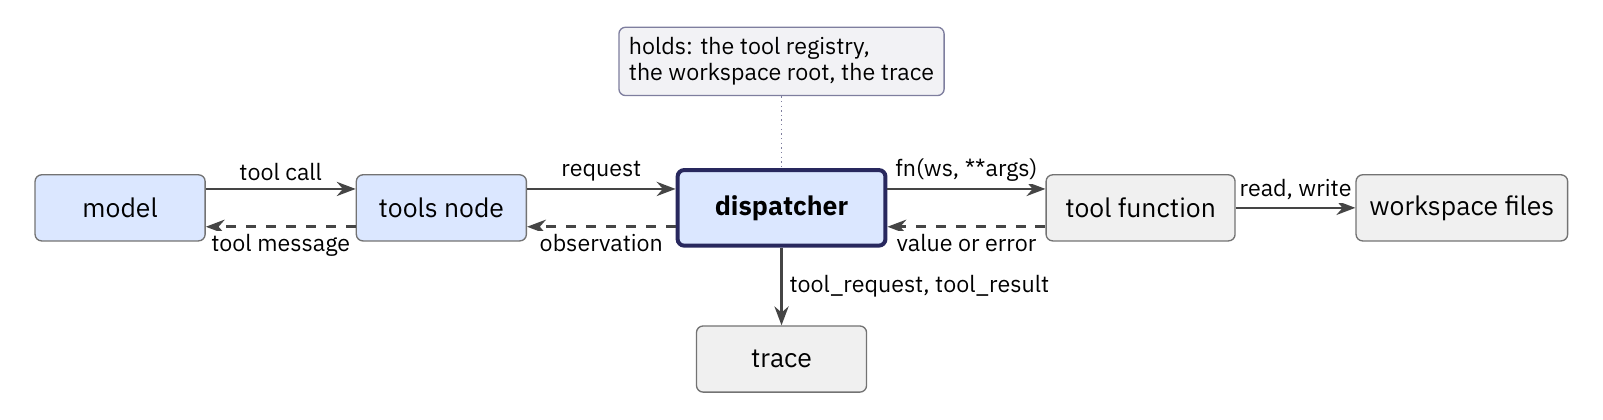
\includegraphics[width=0.9\textwidth]{figures/deck/d9c53fb5c2.png}
  \caption{The dispatcher between the tools node and the tool function. The dispatcher calls the
  tool function with the workspace root and the model's arguments, writes two events to the trace,
  and returns an observation, which reaches the model as a tool message. Only the tool function
  reads or writes the workspace files.}
  \label{fig:dispatcher-role}
\end{figure*}

The model never calls a tool function. It can only request a call, by writing a tool call in its
reply. The dispatcher decides whether the call runs and how. Whatever the model writes, a tool
function runs only when the dispatcher calls it, so every check placed in the dispatcher applies to
every tool call.

\subsection{Binding and the workspace root}
\label{sec:dispatcher-binding}

The dispatcher supplies the workspace root itself and lets the model supply only the other
arguments. \textbf{Binding} is the step that matches the model's arguments to the parameters of the
tool function without calling the function. The dispatcher binds the workspace root to the first
parameter, \demoref{ws}, and matches the model's arguments by name to the parameters that remain.
\Cref{lst:dispatcher-bind} shows the signature of \demoref{read\_file} and the call that performs
the binding.

\begin{lstlisting}[float=tbp, basicstyle=\ttfamily\footnotesize, caption={Illustrative code: the signature of \demoref{read\_file}, and the call with which the dispatcher binds the model's arguments to it.}, label=lst:dispatcher-bind]
def read_file(ws: Path, path: str,
              start: int | None = None,
              end: int | None = None) -> str: ...

# the dispatcher supplies ws before the model's arguments
inspect.signature(function).bind(ws, **args)
\end{lstlisting}

The function \demoref{read\_file} takes the workspace root \demoref{ws}, the path of a file, and an
optional range of lines from \demoref{start} to \demoref{end}. In the last line, \demoref{function}
is the function that the registry returned for the requested name, and \demoref{args} holds the
arguments of the model's tool call. Python's \demoref{inspect.signature(...).bind} checks that a set
of arguments fits a function's parameters, and it does not call the function. If a name matches no
parameter, or a required parameter receives no value, binding fails and the dispatcher refuses the
request. A \textbf{refusal} is the dispatcher's decision not to run a request. The dispatcher
returns the reason to the model as an observation instead, and the run continues
(\cref{sec:dispatcher-refusals}).

A request that names \demoref{ws} fails to bind, because the dispatcher has already supplied that
parameter. The model therefore cannot replace the root against which the tools resolve their paths.
The argument schema also omits \demoref{ws}, so the model is never told that the parameter exists.
The model still chooses the path arguments, so a tool that opens a path must still check it
(\cref{sec:dispatcher-search}).

Binding also explains why the tools read the run's settings, such as its limits, from a module.
Every parameter after the workspace root is a value the model may supply. If a tool took the run's
settings as a parameter, for example a parameter named \demoref{config}, binding would accept a
value for it from the model like any other argument. No argument from the model can reach a value
that the tool reads from a module.

Both choices follow one principle. \textbf{Authority} is the power to decide something about the
run, such as which directory a tool may touch or which limits apply. The model cannot supply
authority it was never given, because the harness supplies those values itself, outside the reach
of the model's arguments.

\subsection{What the model sees and what runs}
\label{sec:dispatcher-definition}

The model sees a tool's definition, and the dispatcher runs the tool's function. The definition
describes the tool's rules, and only the function and the dispatcher's checks enforce them. In
\msa{}, the definition of \demoref{edit} is written as a
separate function, \demoref{edit\_schema}, whose name, parameters and description are converted
into the definition that the model receives. Its body never runs. The dispatcher executes the real
\demoref{edit} instead, so that every call passes through the dispatcher's checks and appears in the
trace.

\Cref{lst:dispatcher-schema} shows the definition of \demoref{edit} in the JSON form in which the
model receives it. The \demoref{description} field states the tool's purpose and its rules. The
\demoref{parameters} field is the argument schema: it lists three required string arguments,
\demoref{path}, \demoref{old} and \demoref{new}. It omits \demoref{ws}, which the dispatcher
supplies. Model providers use slightly
different formats for the same content (\cref{sec:native}).

\begin{lstlisting}[float=tbp, basicstyle=\ttfamily\footnotesize, caption={Illustrative code: the definition of \demoref{edit} as the model receives it, abbreviated.}, label=lst:dispatcher-schema]
{"type": "function",
 "function": {
   "name": "edit",
   "description": "Replace an exact string in a
     file. `old` must appear exactly once in the
     file, so include enough surrounding text to
     make it unique. ...",
   "parameters": {
     "type": "object",
     "properties": {
       "path": {"type": "string"},
       "old":  {"type": "string"},
       "new":  {"type": "string"}},
     "required": ["path", "old", "new"]}}}
\end{lstlisting}

The description tells the model that \demoref{old} must occur exactly once in the file. Only the
body of \demoref{edit} enforces that rule (\cref{lst:dispatcher-edit}). The function counts the
occurrences of \demoref{old} and raises an error, before it writes anything, unless the count is
exactly one. If the sentence were deleted from the description, the rule would still hold. If the
count were deleted from the body, the rule would no longer hold, whatever the description said.

\begin{lstlisting}[float=tbp, basicstyle=\ttfamily\footnotesize, caption={Illustrative code: an excerpt of the function \demoref{edit} that the dispatcher runs.}, label=lst:dispatcher-edit]
def edit(ws, path, old, new):
    target = resolve(ws, path)    # the path check
    body = target.read_text()
    occurrences = body.count(old)
    if occurrences != 1:
        raise ValueError(...)     # nothing written
    target.write_text(body.replace(old, new, 1))
    return {"path": path, "replaced": 1}
\end{lstlisting}

The first line of the body is the path check. The \textbf{path check} accepts a path only if it
resolves to a location inside the workspace root, and raises an exception otherwise. To resolve a
path is to rewrite it as the absolute location it names, so that a step up to a parent directory,
written \texttt{..}, is applied before the comparison. In \msa{}, the path check is the function
\demoref{workspace.resolve}. It is the first step of \demoref{read\_file} and of \demoref{edit}.

\subsection{The dispatch cycle}
\label{sec:dispatcher-cycle}

Each tool call passes through a cycle of operations that the dispatcher controls
(\cref{fig:dispatcher-cycle}):
\be
\item \textbf{Find.} The dispatcher looks the tool's name up in the registry. A name that is not
registered is refused.
\item \textbf{Bind.} The dispatcher binds the arguments to the function's parameters
(\cref{sec:dispatcher-binding}). Arguments that do not bind are refused.
\item \textbf{Check.} The request is checked against the policy. In \msa{}, the policy requires
every path to lie inside the workspace root. The path check enforces it as the first step inside
\demoref{read\_file} and \demoref{edit}, and a path outside the root is refused. A call to
\demoref{search} passes through no such check (\cref{sec:dispatcher-search}).
\item \textbf{Run.} The tool function performs the permitted operation. It returns a value, or it
fails with an error.
\item \textbf{Observe.} The dispatcher records the outcome as an observation and writes a
\demoref{tool\_result} event to the trace. An observation carries the \demoref{ok} flag, the result
or the reason for a failure, and the arguments of the call. The \demoref{ok} flag is true only when
the call succeeded.
\ee

\begin{figure}[htbp]
  \centering
  \begin{adjustbox}{width=\linewidth}
  \begin{tikzpicture}[node distance=4mm,
      op/.style={rnode, text width=41mm, align=left}]
    \node[tnode] (req) {tool request};
    \node[op, below=of req] (find) {\textbf{find} the tool's name in the registry};
    \node[op, below=of find] (bind) {\textbf{bind} the arguments to the function's parameters};
    \node[op, below=of bind] (check) {\textbf{check} that the path lies inside the workspace root};
    \node[op, below=of check] (run) {\textbf{run} the permitted operation};
    \node[op, below=7mm of run, fill=ibmblue!15] (obs) {\textbf{observe}: an observation with
      \texttt{ok}, the result or the reason, and the arguments};
    \node[tnode, below=of obs] (out) {state record, trace event, next model input};
    \draw[flow] (req) -- (find);
    \draw[flow] (find) -- (bind);
    \draw[flow] (bind) -- (check);
    \draw[flow] (check) -- (run);
    \draw[flow] (run) -- node[lab, right=1mm] {result, or error} (obs);
    \draw[flow] (obs) -- (out);
    \coordinate (bus) at ([xshift=-27mm]find.west);
    \draw[back] (find.west) -- node[lab, above=0.5mm] {unregistered tool} (find.west -| bus)
      |- (obs.west);
    \draw[thick, dashed, draw=ibmfg!80] (bind.west) -- node[lab, above=0.5mm]
      {arguments do not bind} (bind.west -| bus);
    \draw[thick, dashed, draw=ibmfg!80] (check.west) -- node[lab, above=0.5mm]
      {path outside the root} (check.west -| bus);
  \end{tikzpicture}
  \end{adjustbox}
  \caption{The dispatch cycle for one tool request. The solid arrows are the path of a permitted
  call. The dashed arrows are the refusals of an unregistered tool, of arguments that do not bind
  and of a path outside the root, and they end in an observation, as a permitted call does.}
  \label{fig:dispatcher-cycle}
\end{figure}

\Cref{lst:dispatcher-cycle} writes the cycle as pseudocode. The comments mark the operations.

\begin{lstlisting}[float=tbp, basicstyle=\ttfamily\footnotesize, caption={Illustrative pseudocode for the dispatch of one tool request.}, label=lst:dispatcher-cycle]
def dispatch(request):
    trace.event("tool_request", request)
    fn = registry.get(request.name)     # find
    if fn is None:
        return refuse("unregistered tool")
    try:
        bind(fn, ws, request.args)      # bind
    except TypeError:
        return refuse("bad arguments")
    try:                                # check + run
        value = fn(ws, **request.args)
    except PathEscape:
        return refuse("outside workspace")
    return observe(value)               # observe
\end{lstlisting}

The listing makes the order of events explicit:
\bi
\item \textbf{The request event.} The first line writes the \demoref{tool\_request} event before any
check, so every request appears in the trace, including the requests that are later refused.
\item \textbf{Find and bind.} A name missing from the registry, or arguments that do not bind, end
the dispatch with a refusal before any tool function is called. Binding signals a mismatch by
raising Python's \demoref{TypeError}.
\item \textbf{Check and run.} The tool function is called with the workspace root and the model's
arguments. \demoref{PathEscape} stands for the exception that the path check raises.
\item \textbf{Refuse and observe.} Each of \demoref{refuse} and \demoref{observe} writes a
\demoref{tool\_result} event and returns an observation. A refusal carries \demoref{ok} false and the
reason. A successful call carries \demoref{ok} true and the result.
\ei
The listing omits the conversion of argument types and the handling of failures inside a tool,
which \cref{sec:dispatcher-refusals} describes.

In \msa{}, the check of policy is not a separate stage of the dispatcher. It is the path check, the
first step inside \demoref{read\_file} and \demoref{edit}. When a path lies outside the root, the
path check raises its exception before the tool reads or writes anything, and the dispatcher turns
that exception into a refusal. For this reason the check and the run share one \texttt{try} block
in the listing, while \cref{fig:dispatcher-cycle} draws them as separate boxes.

Every request ends in an observation, unless an exception that the dispatcher does not expect
interrupts the cycle. Such an exception ends the run without an observation
(\cref{sec:dispatcher-refusals}). The harness stores each observation in the state record
(Lecture~3), and the model reads it in its next input.

\subsection{Refusals}
\label{sec:dispatcher-refusals}

A refused call returns an error to the model as an observation, and the run continues. The
observation of a refusal (\cref{sec:dispatcher-binding}) has its \demoref{ok} flag set to false,
and its result states the reason.

A harness can report a failed call as an exception or as an observation, and the two affect the run
differently:
\bi
\item \textbf{An exception.} An unhandled exception ends the run.
\item \textbf{An observation.} An observation reaches the model, which reads what went wrong and can
revise its request, for example by correcting an argument name or choosing a path inside the
workspace.
\ei
The reactive loop of Lecture~2 depends on observations. The loop works because the model sees the
result of each action, and a refusal is a result that the model can act on.

A \textbf{tool error} is a failure of the tool's operation itself, after the request has passed the
checks. An \demoref{edit} whose \demoref{old} string occurs twice is an example. The operation
cannot tell which occurrence to replace, so the function raises an error before it writes anything
(\cref{sec:dispatcher-definition}). The dispatcher catches the tool errors it expects and returns
each one as an observation with \demoref{ok} false, as it does for a refusal.

A refusal and a tool error differ in what failed. A refusal comes from a check of the request: the
name is not registered, the arguments do not bind, or a path lies outside the workspace root. A
tool error comes from the operation, which could not be carried out on the files as they are. In
\msa{}, the path check and the operation both run inside the tool function. A failed path check
still counts as a refusal, because it checks the request and fails before the tool opens any file.

Binding checks the names of the arguments and their number. It does not check their types. When a
type mismatch is unambiguous, the dispatcher converts the value instead of refusing the request.
This conversion is called \textbf{coercion}. If the model passes the string \texttt{"40"} where the
function expects an integer, the dispatcher converts it to the integer 40. A refusal would spend a
model call only to tell the model that its string should have been a number.

The dispatcher catches only the exceptions it expects, and any other exception ends the run. The
design intends this for failures from which the run cannot recover, such as a trace that cannot be
written. An unexpected exception raised inside a tool also ends the run. For example, the library
that \demoref{search} uses to expand a glob raises an exception when the glob is an absolute path.
The dispatcher does not expect this exception, so the run ends and the model never receives a
refusal.

A \textbf{precondition} is a condition that must be true before a call, for example that
\demoref{old} occurs exactly once in the file. A contract that states only its preconditions leaves
the outcome of a wrong request undefined, as the glob example shows. The contract must also say
what happens when a request violates a precondition: whether the call returns a refusal or a tool
error that the model can read, or raises an exception that ends the run.

\subsection{What each record establishes}
\label{sec:dispatcher-records}

A tool call leaves several records, and each establishes something different about whether the
tool ran. The trace of \msa{} records a \demoref{model\_call} event when a node calls the model, a
\demoref{routing} event after each reply of the controller, when its routing function chooses
between the tools node and \demoref{submit}, and the dispatcher's \demoref{tool\_request} and
\demoref{tool\_result} events. Some moves, such as the return from the tools node to the controller,
have no event of their own (\cref{sec:recap}). \Cref{tab:dispatcher-records} follows one
\demoref{read\_file} call of \msa{}, in which the model reads the file that the alert flags. Its rows run from the model's input to the next model
input, in the order in which the records arise. The rows to compare are the model's response and
the \demoref{tool\_result} event.

\begin{table}[htbp]
  \caption{The records that one \demoref{read\_file} call leaves, in the order in which they arise,
  and what each establishes about the execution of the tool.}
  \label{tab:dispatcher-records}
  \begin{adjustbox}{width=\linewidth}\begin{tabularx}{\linewidth}{@{}L{0.3\linewidth}X@{}}
    \toprule
    \textbf{Record or stage} & \textbf{What it establishes} \\
    \midrule
    \textbf{Model input} & The input contains the available tool definitions. The trace does not
      record this input. \\
    \textbf{Model response and \demoref{model\_call} event} & The model asked to call a tool. The
      request alone does not establish that the tool ran. \\
    \textbf{\demoref{routing} event} & The run went to the tools node because the reply contained a
      tool call. The event records a decision and says nothing about execution. \\
    \textbf{\demoref{tool\_request} event} & The dispatcher received the request and began checking
      it. \\
    \textbf{Dispatcher} & The dispatcher checked the request. A refusal reason appears in
      \demoref{tool\_result}, and no separate event is written for each check. \\
    \textbf{\demoref{tool\_result} event} & With \demoref{ok} true, the function ran and returned.
      The event records the length of the result and omits its text. \\
    \textbf{State and next input} & The harness stores the observation in the state record and adds
      a tool message to the next model input. \\
    \bottomrule
  \end{tabularx}\end{adjustbox}
\end{table}

Between the model's response and the execution of the tool lie the dispatcher's checks, and any of
them could have refused the request. The dispatcher writes a successful \demoref{tool\_result} event
only after the function has returned.

The routing event lies between the model's response and the \demoref{tool\_request} event. As in
Lecture~2, a routing event records one routing decision, and its \demoref{by} field names who
supplied the value that the routing function tested. Here the event records that the run went to the
tools node, and \demoref{by="model"} says that the model's reply, which contained a tool call,
selected that edge. The event records where the run went next. It says nothing about whether any
tool executed.

\subsection{The trace events around one call}
\label{sec:dispatcher-events}

The trace places the dispatcher's two events between the model call that requested the tool and the
model call that sees its result. \Cref{fig:dispatcher-events} follows the same \demoref{read\_file}
call through time, from the controller's model call to the next one. The events appear in this
order:
\bi
\item \textbf{\demoref{model\_call}.} The controller calls the model, and the reply contains a
\demoref{read\_file} call. The event shows that the model asked for the tool.
\item \textbf{\demoref{routing}.} The routing function sends the run to the tools node, because the
model's reply contains a tool call.
\item \textbf{\demoref{tool\_request}.} The dispatcher records the request as it arrived.
\item \textbf{\demoref{tool\_result}.} After finding the tool, binding the arguments and running the
function, whose first step is the path check, the dispatcher records the outcome.
\item \textbf{\demoref{model\_call}.} The next model call receives the tool message that carries the
result.
\ei

\begin{figure*}[t]
  \centering
  \begin{adjustbox}{width=\textwidth}
  \begin{tikzpicture}[x=1mm, y=1mm,
      head/.style={gnode, minimum width=20mm},
      act/.style={rnode, minimum height=5mm, inner sep=2pt, font=\sffamily\scriptsize},
      ev/.style={font=\sffamily\scriptsize, anchor=west, align=left},
      lane/.style={draw=black!25, thin},
      tick/.style={draw=black!30, densely dotted}]
    % lanes
    \node[head, mnode] at (0,0) {model};
    \node[head, mnode] at (32,0) {controller};
    \node[head, mnode] at (64,0) {tools node};
    \node[head, rnode] at (96,0) {dispatcher};
    \node[head, rnode] at (128,0) {\texttt{read\_file}};
    \node[head] at (162,0) {trace};
    \foreach \x in {0,32,64,96,128} \draw[lane] (\x,-4) -- (\x,-90);
    % the model call that requests the tool
    \draw[flow] (32,-10) -- node[lab, above] {messages} (0,-10);
    \draw[back] (0,-17) -- node[lab, above] {reply: a \texttt{read\_file} call} (32,-17);
    \draw[tick] (32,-17) -- (150,-17);
    \node[ev] at (150,-17) {\texttt{model\_call}\\[-1pt]\textcolor{black!60}{the model asked}};
    % routing
    \draw[flow] (32,-26) -- node[lab, above] {route: tools (by the model)} (64,-26);
    \draw[tick] (64,-26) -- (150,-26);
    \node[ev] at (150,-26) {\texttt{routing}\\[-1pt]\textcolor{black!60}{the decision}};
    % the dispatcher receives the request
    \draw[flow] (64,-35) -- node[lab, above] {request} (96,-35);
    \draw[tick] (96,-35) -- (150,-35);
    \node[ev] at (150,-35) {\texttt{tool\_request}\\[-1pt]\textcolor{black!60}{the request arrived}};
    % find, bind, run
    \node[act] at (96,-43) {find, bind};
    \draw[flow] (96,-50) -- node[lab, above] {run} (128,-50);
    \node[act] at (128,-56) {path check, then read};
    \draw[back] (128,-62) -- node[lab, above] {file text} (96,-62);
    \draw[tick] (96,-68) -- (150,-68);
    \node[act] at (96,-68) {observe};
    \node[ev] at (150,-68) {\texttt{tool\_result}\\[-1pt]\textbf{the function ran}};
    % the result returns to the model
    \draw[back] (96,-74) -- node[lab, above] {observation} (64,-74);
    \draw[back] (64,-80) -- node[lab, above] {tool message} (32,-80);
    \draw[flow] (32,-86) -- node[lab, above] {messages and tool message} (0,-86);
    \draw[tick] (32,-86) -- (150,-86);
    \node[ev] at (150,-86) {\texttt{model\_call}\\[-1pt]\textcolor{black!60}{the next call sees the result}};
  \end{tikzpicture}
  \end{adjustbox}
  \caption{The trace events around one \demoref{read\_file} call, in time order from top to bottom.
  The controller and the routing function write the \demoref{model\_call} and \demoref{routing}
  events, and the dispatcher writes \demoref{tool\_request} and \demoref{tool\_result}. Only the
  \demoref{tool\_result} event shows that the function ran and returned.}
  \label{fig:dispatcher-events}
\end{figure*}

The dispatcher writes the \demoref{tool\_request} and \demoref{tool\_result} events. It
writes no event for finding the tool, binding the arguments or checking the path. A refusal appears
only as the reason recorded in the \demoref{tool\_result} event. The \demoref{model\_call} and
\demoref{routing} events are written once for each reply of the controller. A reply with two tool calls
therefore produces one \demoref{model\_call} event, one \demoref{routing} event, and two pairs of
\demoref{tool\_request} and \demoref{tool\_result} events.

\subsection{Complete mediation}
\label{sec:dispatcher-mediation}

A check protects a resource only if every route to the resource passes through the check. The model
requests an action, and before executing it the harness checks whether the action is permitted. A
\textbf{guard} is the component that makes such a check: it decides whether an access to a protected
resource is permitted. Lecture~3 used the word for the guard of a transition, the condition under
which the state machine takes a transition. That guard chooses which edge the run follows. The
access guard decides whether a request may reach a resource. From here on, guard means the access
check.

\begin{definition}[Complete mediation]
\label{def:dispatcher-mediation}
``To attempt to secure this resource, server needs to check all accesses to the resource.
`Complete mediation.' Server will put a `guard' in place to mediate every request for this
particular resource. Only way to access the resource is to use the guard.''~\citep{mit6033-lec20}
\end{definition}

\textbf{Complete mediation} means that every request for a protected resource passes
through a guard. In \msa{}, the protected resources are the files, the requests are tool calls, and
the guard for a path is the path check. Complete mediation is a property of all the routes to a
resource together. A correct check provides it only if no route bypasses the check.

A harness can lose complete mediation without any change to its existing check. A new tool may reach
the files through code that never calls the path check. A glob may also expand into paths that no
check has examined, because the tool opens whatever files the pattern matches. In both cases the
existing check is still correct, and it is bypassed. A guard protects a resource only where it is
invoked, so every route by which a tool can reach the resource needs a check.

Complete mediation leaves open whether the policy is right and whether the model's claims are
true:
\bi
\item \textbf{The policy itself.} Checking every request establishes that the policy is applied to
every request. The policy may still contain errors, for example a rule that permits a path it
should refuse.
\item \textbf{Claims by the model.} A model's request, or its claim that an action produced a
result, does not establish that the harness performed the action. A model can write such text
without any tool having run. Only the records that the harness writes, such as the
\demoref{tool\_result} event, show what the harness executed (\cref{sec:dispatcher-records}).
\ei

\subsection{The actors of the harness}
\label{sec:dispatcher-actors}

Before asking which part of \msa{} enforces each guarantee, we name the parts that could. We call each such part an \textbf{actor}: the model and the parts of the harness.
\msa{}, in the planning version that Lecture~3 studied, has the nodes \demoref{plan},
\demoref{controller}, \demoref{tools}, \demoref{submit} and \demoref{validate}. The \textbf{model
nodes} are the nodes that call the model: \demoref{plan}, \demoref{controller} and
\demoref{validate}.

\Cref{tab:dispatcher-actors} lists the actors and the role of each. Note which actors hold no
authority or only pass calls on, because the next subsection rules them out.

\begin{table}[htbp]
  \caption{The actors of \msa{}, the model and the parts of its harness, and the role of each.}
  \label{tab:dispatcher-actors}
  \begin{adjustbox}{width=\linewidth}\begin{tabularx}{\linewidth}{@{}L{0.3\linewidth}X@{}}
    \toprule
    \textbf{Actor} & \textbf{Role} \\
    \midrule
    \textbf{The model} & Proposes tool calls and supplies their arguments. It holds no
      authority. \\
    \textbf{The model nodes} & \demoref{plan}, \demoref{controller} and \demoref{validate} call the
      model, and each checks the call budget first. \\
    \textbf{The tools node} & Passes every call of a reply to the dispatcher, in order. \\
    \textbf{The dispatcher} & Finds the tool in the registry, binds the arguments, and turns every
      expected refusal into an observation. \\
    \textbf{The tool function} & Performs the operation. \demoref{read\_file} and \demoref{search}
      read, and \demoref{edit} is the only writer. \\
    \textbf{The path check} & Accepts a path only if it lies inside the workspace root. \\
    \textbf{The workspace} & A disposable copy of the files that the agent may read and write. \\
    \textbf{The trace} & Records events of the run, such as model calls, tool requests and results,
      many routing decisions and a terminal event. It stops nothing. \\
    \bottomrule
  \end{tabularx}\end{adjustbox}
\end{table}

\subsection{Which actor enforces each guarantee}
\label{sec:dispatcher-enforcers}

A guarantee is enforced by the actor whose code stops a violation before it happens. For each
guarantee below, we name that actor and explain why the other plausible actors do not enforce it.
\bi
\item \textbf{Only registered tools run.} The dispatcher enforces this guarantee. It looks the
tool's name up in the registry before it calls any function, and it refuses a name it does not
find, listing the registered tools so that the model can correct its request. The model cannot
enforce the guarantee, because it holds no authority and may request any name, including one that
was never defined. The tools node passes every call to the dispatcher without examining it. A tool
function cannot enforce it, because an unregistered tool has no function to call. A tool absent
from the registry cannot run, whatever tool definitions the model was given.
\item \textbf{Arguments match the tool's parameters.} The dispatcher enforces this guarantee. It
binds the arguments before calling the function, so a wrong argument name becomes a refusal that the
model can read, and it coerces unambiguous type mismatches. The model supplies the arguments, so it
is the source of a mismatch and cannot be its check. A tool function cannot enforce the guarantee
either. A call whose argument names do not fit the function's parameters fails before the body of
the function runs, so no check inside the tool can catch the mistake. The path check examines paths
and nothing else.
\item \textbf{Writes stay inside the workspace.} The \demoref{edit} tool enforces this guarantee,
through the path check. \demoref{edit} is the only writer, and its first step is the path check. The
dispatcher turns the path check's exception into a refusal. It does not examine paths itself. The
model nodes call the model and check the budget. They never inspect tool arguments. The
workspace is a copy, so a write inside it leaves the original code base unchanged. A copy cannot
stop a write aimed at a path outside it.
\item \textbf{No model call happens after the budget is exhausted.} The model nodes enforce this
guarantee. Each of \demoref{plan}, \demoref{controller} and \demoref{validate} checks the budget
before it calls the model, which is the admission check of Lecture~3. When the count of model calls
has reached the budget, the node ends the run instead of calling the model. The dispatcher and the
tools node handle tool calls and never call the model. The trace records events and stops nothing,
so it could show an extra model call only after the call had been made.
\ei

The check for writes sits inside a tool, and the other checks sit outside the tools. Placing a check
inside the tool is acceptable when it runs before the protected effect. The path check runs before
\demoref{edit} writes anything, so a refused write never happens.

\subsection{The search tool reads outside the workspace}
\label{sec:dispatcher-search}

The path check confines the tools that call it, and \demoref{search} does not call it, so
\demoref{search} can read files outside the workspace. Requests constructed to test the path check,
and sent to the dispatcher, show the difference:
\bi
\item \textbf{A refused read.} A \demoref{read\_file} request with the path
\texttt{../../etc/passwd}, which climbs two directories above the workspace root and so names a
file outside it, is refused. The dispatcher returns an observation with \demoref{ok} false and the reason. The trace
holds a \demoref{tool\_request} event and a failed \demoref{tool\_result} event that records the
reason.
\item \textbf{A read that is not refused.} A \demoref{search} request whose glob begins with
\texttt{../} climbs into a sibling directory of the workspace. The tool reads the files there and
reports success, with \demoref{ok} true.
\ei

The two requests reach the files by different routes. \demoref{read\_file} and \demoref{edit} pass
every path through the path check. \demoref{search} applies its glob to the workspace root and opens
every file that the glob matches, without the path check. A glob that climbs out of the root matches
files outside it, and nothing examines them.

This is a failure of complete mediation (\cref{sec:dispatcher-mediation}). The path check itself is
correct, and \demoref{search} is a route to the files that does not pass through it. A read outside
the workspace can expose files that the run was never meant to see.

The repair is to apply the path check to every file that \demoref{search} matches, before the tool
opens it. With this repair, every route by which a tool opens a file passes through the same guard.
Writes are already confined, because \demoref{edit} is the only writer and every write passes
through the path check.

\subsection{Where each guarantee is enforced}
\label{sec:dispatcher-guarantees}

\Cref{tab:dispatcher-guarantees} collects the guarantees of the harness and the place where each
one is enforced. The row to read is the one about reads. It names the missing path check, which
leaves that guarantee without an enforcer.

\begin{table}[htbp]
  \caption{The guarantees of the harness of \msa{} and where each is enforced. Reads are not
  confined to the workspace.}
  \label{tab:dispatcher-guarantees}
  \begin{adjustbox}{width=\linewidth}\begin{tabularx}{\linewidth}{@{}L{0.36\linewidth}X@{}}
    \toprule
    \textbf{Guarantee} & \textbf{Where it is enforced} \\
    \midrule
    \textbf{Only registered tools run} & The dispatcher checks the registry before calling a tool. \\
    \textbf{Arguments match the tool's parameters} & The dispatcher binds the arguments and converts
      unambiguous type mismatches. \\
    \textbf{Writes stay inside the workspace} & The \demoref{edit} tool, the only writer, checks
      paths with the path check. \\
    \textbf{Reads stay inside the workspace} & Not enforced. The glob of \demoref{search} bypasses
      the path check. \\
    \textbf{No model call after the budget is exhausted} & Each model node checks the budget before
      calling the model. \\
    \bottomrule
  \end{tabularx}\end{adjustbox}
\end{table}

The dispatcher enforces the guarantees about registered tools and arguments. The \demoref{edit}
tool enforces the guarantee about writes, and the model nodes enforce the budget. Every enforcer in
the table is code that runs before the effect it protects. None of them is a sentence in a prompt or
in a tool's description, which the model may ignore (\cref{sec:dispatcher-contract}).

A guarantee holds only where an actor enforces it, so a table that names the enforcer of each
guarantee also shows where an enforcer is missing.

\subsection*{Key points}
\bi
\item The model receives only a tool's definition, and only code in the tool function or the
dispatcher enforces the constraints of the tool's contract.
\item The dispatcher receives each tool request, finds the tool, binds the arguments, calls the tool
function and returns an observation, and the model never calls a tool function itself.
\item The dispatcher supplies the workspace root when it binds the arguments, and the tools read the
run's settings from a module, so the model cannot supply authority it was never given.
\item A refusal returns to the model as an observation with \demoref{ok} false, so the model can
revise its request, while an unhandled exception ends the run.
\item A tool call in the model's response shows only that the model asked, and the successful
\demoref{tool\_result} event that the dispatcher writes is the record that shows the function ran
and returned.
\item Complete mediation requires every route to a protected resource to pass a guard, and checking
every request still cannot show that the policy itself is correct.
\item The dispatcher enforces that only registered tools run and that arguments bind, each model node
enforces the budget before it calls the model, and the path check inside \demoref{edit} keeps writes
in the workspace, while reads escape it because \demoref{search} opens the files its glob matches
without that check.
\ei
